\textbf{Revised \today , at \currenttime}

% \providecommand{\comment}[1]{\textbf{[#1]}}

\section{Introduction}


Since the discovery of long-lived oscillations in cross peaks of the two-dimensional electronic spectrum of the Fenna-Matthews-Olsen (FMO) complex~\cite{FMO1}, there has been a great deal of interest because the observed oscillations could mean that photosynthetic chlorophylls were keeping a stable superposition of electronic-excited-states for much longer than a chaotic biological environment was expected to allow ~\cite{FMO2,Panitchayangkoon2011,Lambert2012}.
%
A long-lived electronic superposition (coherence) can have positive consequences for energy transfer rates and efficiencies~\cite{FMO1}, so biological protection against electronic decoherence would be a profoundly interesting result of natural selection--one that we might hope to emulate. There is further suggestion that the FMO and other photosynthetic complexes may have an optimal dephasing rate for energy transfer efficiency between perfect coherence and strong dephasing, both of which are sub-optimal ~\cite{energyTransfer} ~\cite{Panitchayangkoon2011,Fidler2013,Collini2010}.  There is also great interest in being able to mimic these evolution-tuned efficiencies for artificial designs ~\cite{Creatore2013}.

The assignment of the off-diagonal oscillations to electronic effects is, however, disputed, as vibrations can cause similar signatures.  While much useful work has been done to pinpoint the  unique signatures of electronic coherence and the unique signatures of vibrational coherence in a two-dimensional electronic spectroscopy experiment ~\cite{FMO2,mech2,mech3,mech1,mech4,Halpin2014,Chenu2013}, such signatures remain disputed, and a simpler, unambiguous tool to distinguish electronic from vibrational coherences is valuable.

Yuen-Zhou et al.\ proposed such an experiment \cite{witness}, which aims to give a concrete yes or no answer (called a witness in the language of quantum information~\cite{Chuang2005}) to the question of whether a given coherent oscillation has electronic character.  That work proposed using only a one dimensional pump-probe experiment in the impulsive (i.e., ultrashort pulse) limit.  They showed that for impulsive pulses, there are no oscillations in the frequency-integrated pump probe signal when a system has only vibrational coherences. Oscillations in the pump-probe signal  are a witness for electronic coherence.  Thus for the rest of this paper, we will refer to the proposed procedure as ``The Witness''.

The effects of pulse widths on pump-probe spectroscopy had been studied previously~\cite{pulseWidth} but the proposed witness uniquely suggested using pulse width as an independent variable in an experiment, which should be feasible given developments in two-dimensional spectroscopy using pulse-shaping devices~\cite{pulse1,pulse2,Stock1988,Stock1992}.

Johnson et al.  ~\cite{allanWitness} showed that the witness procedure works for finite-duration pulses and proposed to use several such pulse durations to extrapolate to the impulsive limit. Generally speaking, if the oscillations in a pump probe experiment approach zero as the pulse duration approaches 0, then there is no electronic coherence.  If, however, the oscillations increase as the pulse duration approaches 0, then there is an electronic coherence.

An essential assumption of Refs.~\cite{witness,allanWitness} is the Condon approximation, that transition dipoles have no variation with respect to nuclear coordinate ~\cite{Condon,FranckCondon}. This approximation is widely used in molecular spectroscopy, and there are also well-known systems in which non-Condon effects are highly important \cite{photosyntheticKappa,MavrosNonCondon,hellerGraphene,Hockett2011}. In this work, we show how well the witness protocol can tolerate a violation of the Condon approximation. We show that for systems with small electron-vibration coupling, quantified by the Huang-Rhys factor $S$, the witness protocol can give false-positive results even with small non-Condon effects. For larger values of $S$, where the vibrational coherence is more visible in optical experiments, the witness protocol is robust to larger non-Condon effects, with a small modification to the interpretation of the data. We quantify the parameter range in which the protocol is expected to work.


To test the effect of transition dipole variation on the witness experiment, we construct the simplest possible system with vibrational effects but no electronic coherence and then simulate pump probe experiments.  Our system of choice has two electronic levels and a single harmonic vibrational level. This system is the same as that studied in Refs.~\cite{witness,allanWitness}, with the addition of non-Condon effects in the transition dipole.

\section{Methods}

We study a model system with two electronic levels, labelled $\ket{g}$ and $\ket{e}$, coupled to a single harmonic vibrational mode. The frequency of the vibration is $\omega_\gamma$, $\omega_\epsilon$ when the system is in the state $\ket{g}$, $\ket{e}$, respectively, giving a Hamiltonian
\begin{align}
	H_0 &=  \sum_n \hbar \omega_{\gamma}  \left(n + \frac{1}{2} \right)  \ket{n_{\gamma}}\ket{g}\bra{g} \bra{n_{\gamma}} \\
   &+ \sum_m \left(  \hbar \omega_{\epsilon}  \left(m + \frac{1}{2} \right) + \omega_e \right)  \ket{m_{\epsilon}} \ket{e}\bra{e} \bra{m_{\epsilon}}.
\end{align}
Greek indices correspond to the vibrational states and the roman indices correspond to the electronic states.  The ground-state vibrational wavefunctions $\langle x \ket{n_\gamma}$ are centered at vibrational coordinate $x=0$ while the excited-state vibrational wavefunctions $\langle x \ket{m_\epsilon}$ are centered at $x=\delta x$, giving a Huang-Rhys factor of $S=\frac{\omega_\gamma \omega_\epsilon(\delta x)^2}{\hbar (\omega_\gamma+\omega_\epsilon)}$.

We consider the transition dipole to be aligned with the optical pulse polarizations, for simplicity, with a transition dipole
\begin{align}
	\hat{\mu}(x) &= \mu (x)  \left( \ket{e}\bra{g} + \ket{g} \bra{e} \right).
\end{align}
In the Condon approximation, $\mu(x)=\mu_0$ is a constant. In the spirit of keeping things as simple as possible to demonstrate the effect of transition dipole variations, we consider a linear form of $\mu(x)$:
\begin{align}
	\mu(x) &= \mu_0\left( 1 +  \kappa x \right)
\end{align}
To make $\kappa$ comparable for different values of $\delta x$, we define also the dimensionless quantity $\lambda=\delta x \kappa$.
The quantity $\lambda$ has the useful property that above $\lambda=1$, the variation of $\mu$ as the system moves from the ground- to excited-state equilibrium position becomes larger than the mean value $\mu_0$.  As a reference, in C-phycocyanin, $\kappa$ has been calculated to be approximately 0.3 and $\lambda$ to be approximately 0.1 \cite{photosyntheticKappa}.

We simulate Pump Probe spectroscopy using ideal Gaussian laser pulses, which differ only in their pulse durations and arrival times.  This means that both of our pulses (labeled pu for pump and pr for probe) will have the form:
\begin{align}
	E_{\text{pu}} &= \frac{E_0}{\sqrt{2 \pi \sigma^2}} e^{-\frac{t^2}{2 \sigma^2} } \left[ e^{-i \omega_c t} + e^{i \omega_c t} \right]\\
	E_{\text{pr}} &= \frac{E_0}{\sqrt{2 \pi \sigma^2}} e^{-\frac{\left(t-T\right)^2}{2 \sigma^2} } \left[ e^{-i \omega_c \left(t-T\right)} + e^{i \omega_c \left(t-T\right)} \right]
\end{align}
We normalize the pulses as in Ref.~\cite{allanWitness} to keep the integral of the absolute value of the electric field constant across with varying pulse widths.  The pulse's central frequency $\omega_c$ is always tuned to the strongest absorption transition in the simulated system and the pulse width $\sigma$ is our main experimental independent variable.

In the rotating wave approximation, it is helpful to further split the laser pulses into positive frequency excitation pulses:
\begin{align}
	E_{\text{pu}+}(t) &= \frac{E_0}{\sqrt{2 \pi \sigma^2}} e^{-\frac{t^2}{2 \sigma^2} } e^{-i \omega_c t} \\
	E_{\text{pr}+}(t) &= \frac{E_0}{\sqrt{2 \pi \sigma^2}} e^{-\frac{\left(t-T\right)^2}{2 \sigma^2} }  e^{-i \omega_c \left(t-T\right)}
\end{align}
and negative frequency relaxation pulses:
\begin{align}
	E_{\text{pu}-}(t) &= \frac{E_0}{\sqrt{2 \pi \sigma^2}} e^{-\frac{t^2}{2 \sigma^2} } e^{i \omega_c t} \\
	E_{\text{pr}-}(t) &= \frac{E_0}{\sqrt{2 \pi \sigma^2}} e^{-\frac{\left(t-T\right)^2}{2 \sigma^2} }  e^{i \omega_c \left(t-T\right)}
\end{align}
Assuming that the system begins in state $\ket{\psi_0}$, the first order perturbative wavepacket after one interaction with pulse $Q$ is
\begin{align}
	\ket{\psi_{Q} (t)}  &= -\frac{i}{\hbar} \int_{-\infty}^{t} U(t, \tau) E_{Q}(\tau) \hat{\mu}(x) \ket{\psi_0 (\tau)} d \tau.
\end{align}
A subsequent interaction with pulse $P$, which could be the same pulse, gives the second-order perturbative wavepacket
\begin{align}
	\ket{\psi_{Q, P} (t)}  &= -\frac{i}{\hbar} \int_{-\infty}^{t} U(t, \tau) E_P (\tau) \hat{\mu}(x) \ket{\psi_Q (\tau)} d \tau.
\end{align}
Assuming an ensemble of identical systems distributed over a volume larger than the pulse wavelength, contributions to the pump-probe signal require phase matching. In the rotating wave approximation, these perturbative wavepackets allow construction of the pump probe signal $S_{PP}(T)$ as
\begin{align*}
	E_{GSB1} (t, T) &=  i \bra{\psi_{0} (t)} \hat{\mu} (x) \ket{\psi_{\text{pu+, pu-, pr+}} (t, T)}\\
	E_{ESA} (t, T) &=  i \bra{\psi_{\text{pu+}} (t)} \hat{\mu} (x) \ket{\psi_{\text{pu+, pr+}} (t, T)}\\
	E_{GSB2} (t, T) &=  i \bra{\psi_{\text{pu+, pr-}} (t, T)} \hat{\mu} (x) \ket{\psi_{\text{pu+}} (t)}\\
	E_{SE} (t, T) &=  i \bra{\psi_{\text{pu+, pu-}} (t)} \hat{\mu} (x) \ket{\psi_{\text{pr+}} (t, T)} \\
	S_{i} (T) &= 2 \text{Re} \left[ \int E^*_{\text{pr+}} (t) E_i (t, T) dt  \right] \\
	S_{PP} (T) &= S_{GSB1} (T) + S_{GSB2} (T) + S_{ESA} (T) + S_{SE} (T) \\
	\tilde{S}(\Omega) &= \int S_{PP} (T) e^{i \Omega T} d T,\\
	\Gamma &= \int |S_{PP}(T)-\bar{S}_{PP}|^2 dT
\end{align*}
where $t$ is the laboratory time, $T$ is the time delay between the pump and probe pulses. The main object investigated in this work is $\tilde{S}(\Omega)$, the Fourier transform of $S_{PP}(T)$. When $\Omega$ is chosen equal to the vibrational frequency, we explore the changing amplitude of $\tilde{S}(\Omega)$ with pulse duration $\sigma$ for a range of systems with varying Huang-Rhys factors $S$ and non-Condonicities $\kappa$.

We calculate these quantities using time-domain wavepacket propagation, as described previously \cite{Mukamel1995,UFSwavepackets,Tannor2007,technique}.  In this work, we consider only systems with a single electronic excited state, so they have no excited-state electronic coherence. All oscillatory effects in the pump-probe signal are vibrational, so we want to show when the modified witness successfully characterizes these oscillations as vibrational in origin. In all simulations, we choose the central frequency of the optical pulses to be resonant with the strongest transition in the calculated absorption spectrum. We begin with initial states in the lowest-energy vibrational state of the ground state manifold and do not consider thermal or orientational averaging effects, which we do not believe are important for the present study. We do not consider dephasing or inhomogeneous broadening processes.

If we consider the impulsive limit, then we can show that thethe Pump-Probe signals simplfy to:
\begin{align}
	S_{GSB2} &=  E_0^4 \sum_{k}   \cos \left[  \omega_{\gamma}  \left(   k - \eta \right) T \right]  \left(  \bra{\eta_{\gamma}}  \mu^2 (x) \ket{k_{\gamma}} \right)^2 \\
	S_{SE} &= E_0^4 \sum_{j, l}   \cos  \left[\omega_{\epsilon}  \left(   j - l \right) T \right]   \\
	&\times \bra{\eta_{\gamma}}  \mu (x) \ket{j_{\epsilon}} \bra{j_{\epsilon}}  \mu^2 (x) \ket{l_{\epsilon}} \bra{l_{\epsilon}}  \mu (x) \ket{\eta_{\gamma}}   \\
	S_{ESA} &= 0 \\
	S_{GSB1} &=  E_0^4 \sum_{k}  \cos  \left[ \omega_{\gamma}  \left(   k - \eta \right) T  \right]   \left(  \bra{\eta_{\gamma}}  \mu^2 (x) \ket{k_{\gamma}} \right)^2
\end{align}
which because the vibrational states are eigenfunctions, this will be zero unless $\mu(x)$ is non-constant.  So we do expect oscillations at the impulsive limit for non-Condon systems, but we will address the question of how they approach the impulsive limit numerically.

\begin{figure}
   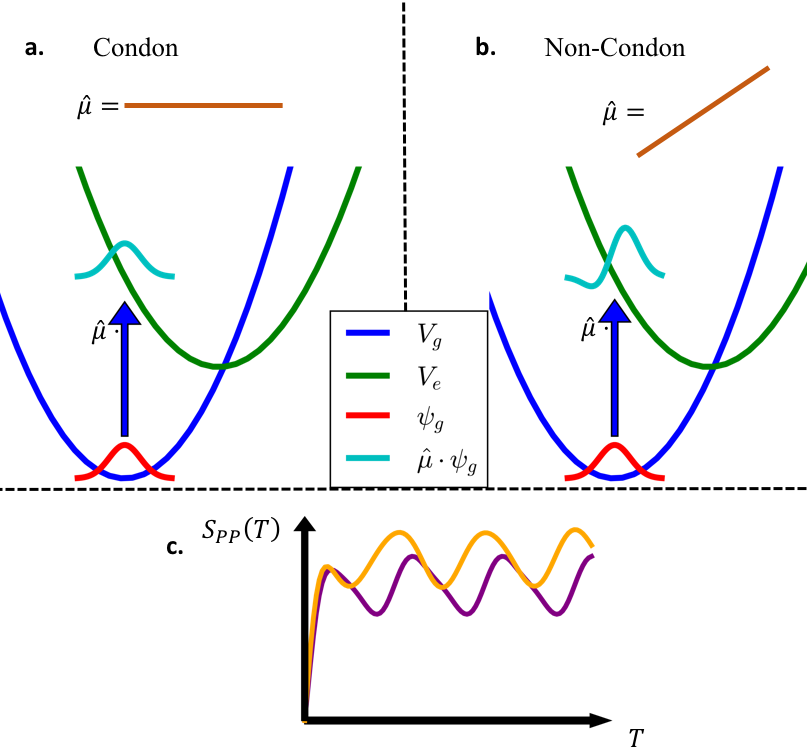
\includegraphics[width=1.0\columnwidth]{excitation_figure.png}
   \caption{In the case where there is no transition dipole variation, when the transition dipole operator is applied (with an impulsive pulse), the ground state wavepacket's shape is perfectly replicated as seen in a.  If, however, we introduce a linear variation, the wavepacket's shape is distorted as we see in b.  THis distortion is, in itself, a change in the vibrational coherence which manifests as a demonstrable difference in the pump probe signal as seen in c and could.  What is not clear is how the the signal changes as the pulse width changes for different transition dipole slopes, so we set out to investigate and see if this change keeps the protocol for electronic coherence detection proposed in ~\cite{witness,allanWitness} from working properly.  }
	\label{fig:physicalIllustration}
\end{figure}


\section{Results and Discussion}

We can consider a variety of model systems, characterized by their vibrational frequencies $\omega_{\gamma}$, $\omega_{\epsilon}$,  Huang-Rhys factor $S$, and non-Condonicity $\lambda$.  For the commonly considered case with $\omega_\gamma\approx\omega_\epsilon$, we show that the witness protocol breaks down for the smallest values of $S$ but is robust for a larger range of $\lambda$ when $S$ is larger. We begin by considering the smallest values of $S$, where the witness is broken, and then consider larger values of $S$ and propose a modified protocol that remains robust even in the presence of some non-Condonicity. For strongly non-Condon transition dipoles, the witness does not work at any $S$.  For specificity, we consider $\omega_{\gamma} = \omega_{\epsilon}= 640 \text{cm}^{-1}$, but all timescales can be easily scaled for any other vibrational frequency of interest.

The worst case scenario for the witness protocol occurs when $S=0$. In that limit, in the Condon-approximation with $\omega_{\gamma} = \omega_{\epsilon}$, the only allowed optical transition is the 0-0 transition, from the lowest vibrational state of the ground state to the lowest vibrational state of the excited state. There is no coherence of any variety, so there is no oscillation in the pump-probe signal, and $\tilde{S}_{PP}(\omega_\epsilon)=0$ always. Even in the Condon approximation, this case is difficult  for the witness protocol, as the signal is independent of pulse duration $\sigma$, rather than monotonically decreasing as $\sigma$ is decreased. This case does, however, illustrate the effects of a non-Condon transition dipole.

In the non-Condon case, the 0-0 and 0-1 transitions are both allowed, producing a vibrational coherence in the singly-excited manifold and a nonzero $\tilde{S}_{PP}(\omega_\epsilon)$. This oscillatory pump-probe signal becomes stronger as $\sigma$ becomes smaller, which looks qualitatively similar to the case of a Condon electronic coherence, as shown for several values of $\kappa$ in Fig.\ \ref{fig:tunedZero}. That is, this witness technique cannot distinguish an electronic coherence from a non-Condon vibrational-only system.

\begin{figure}
   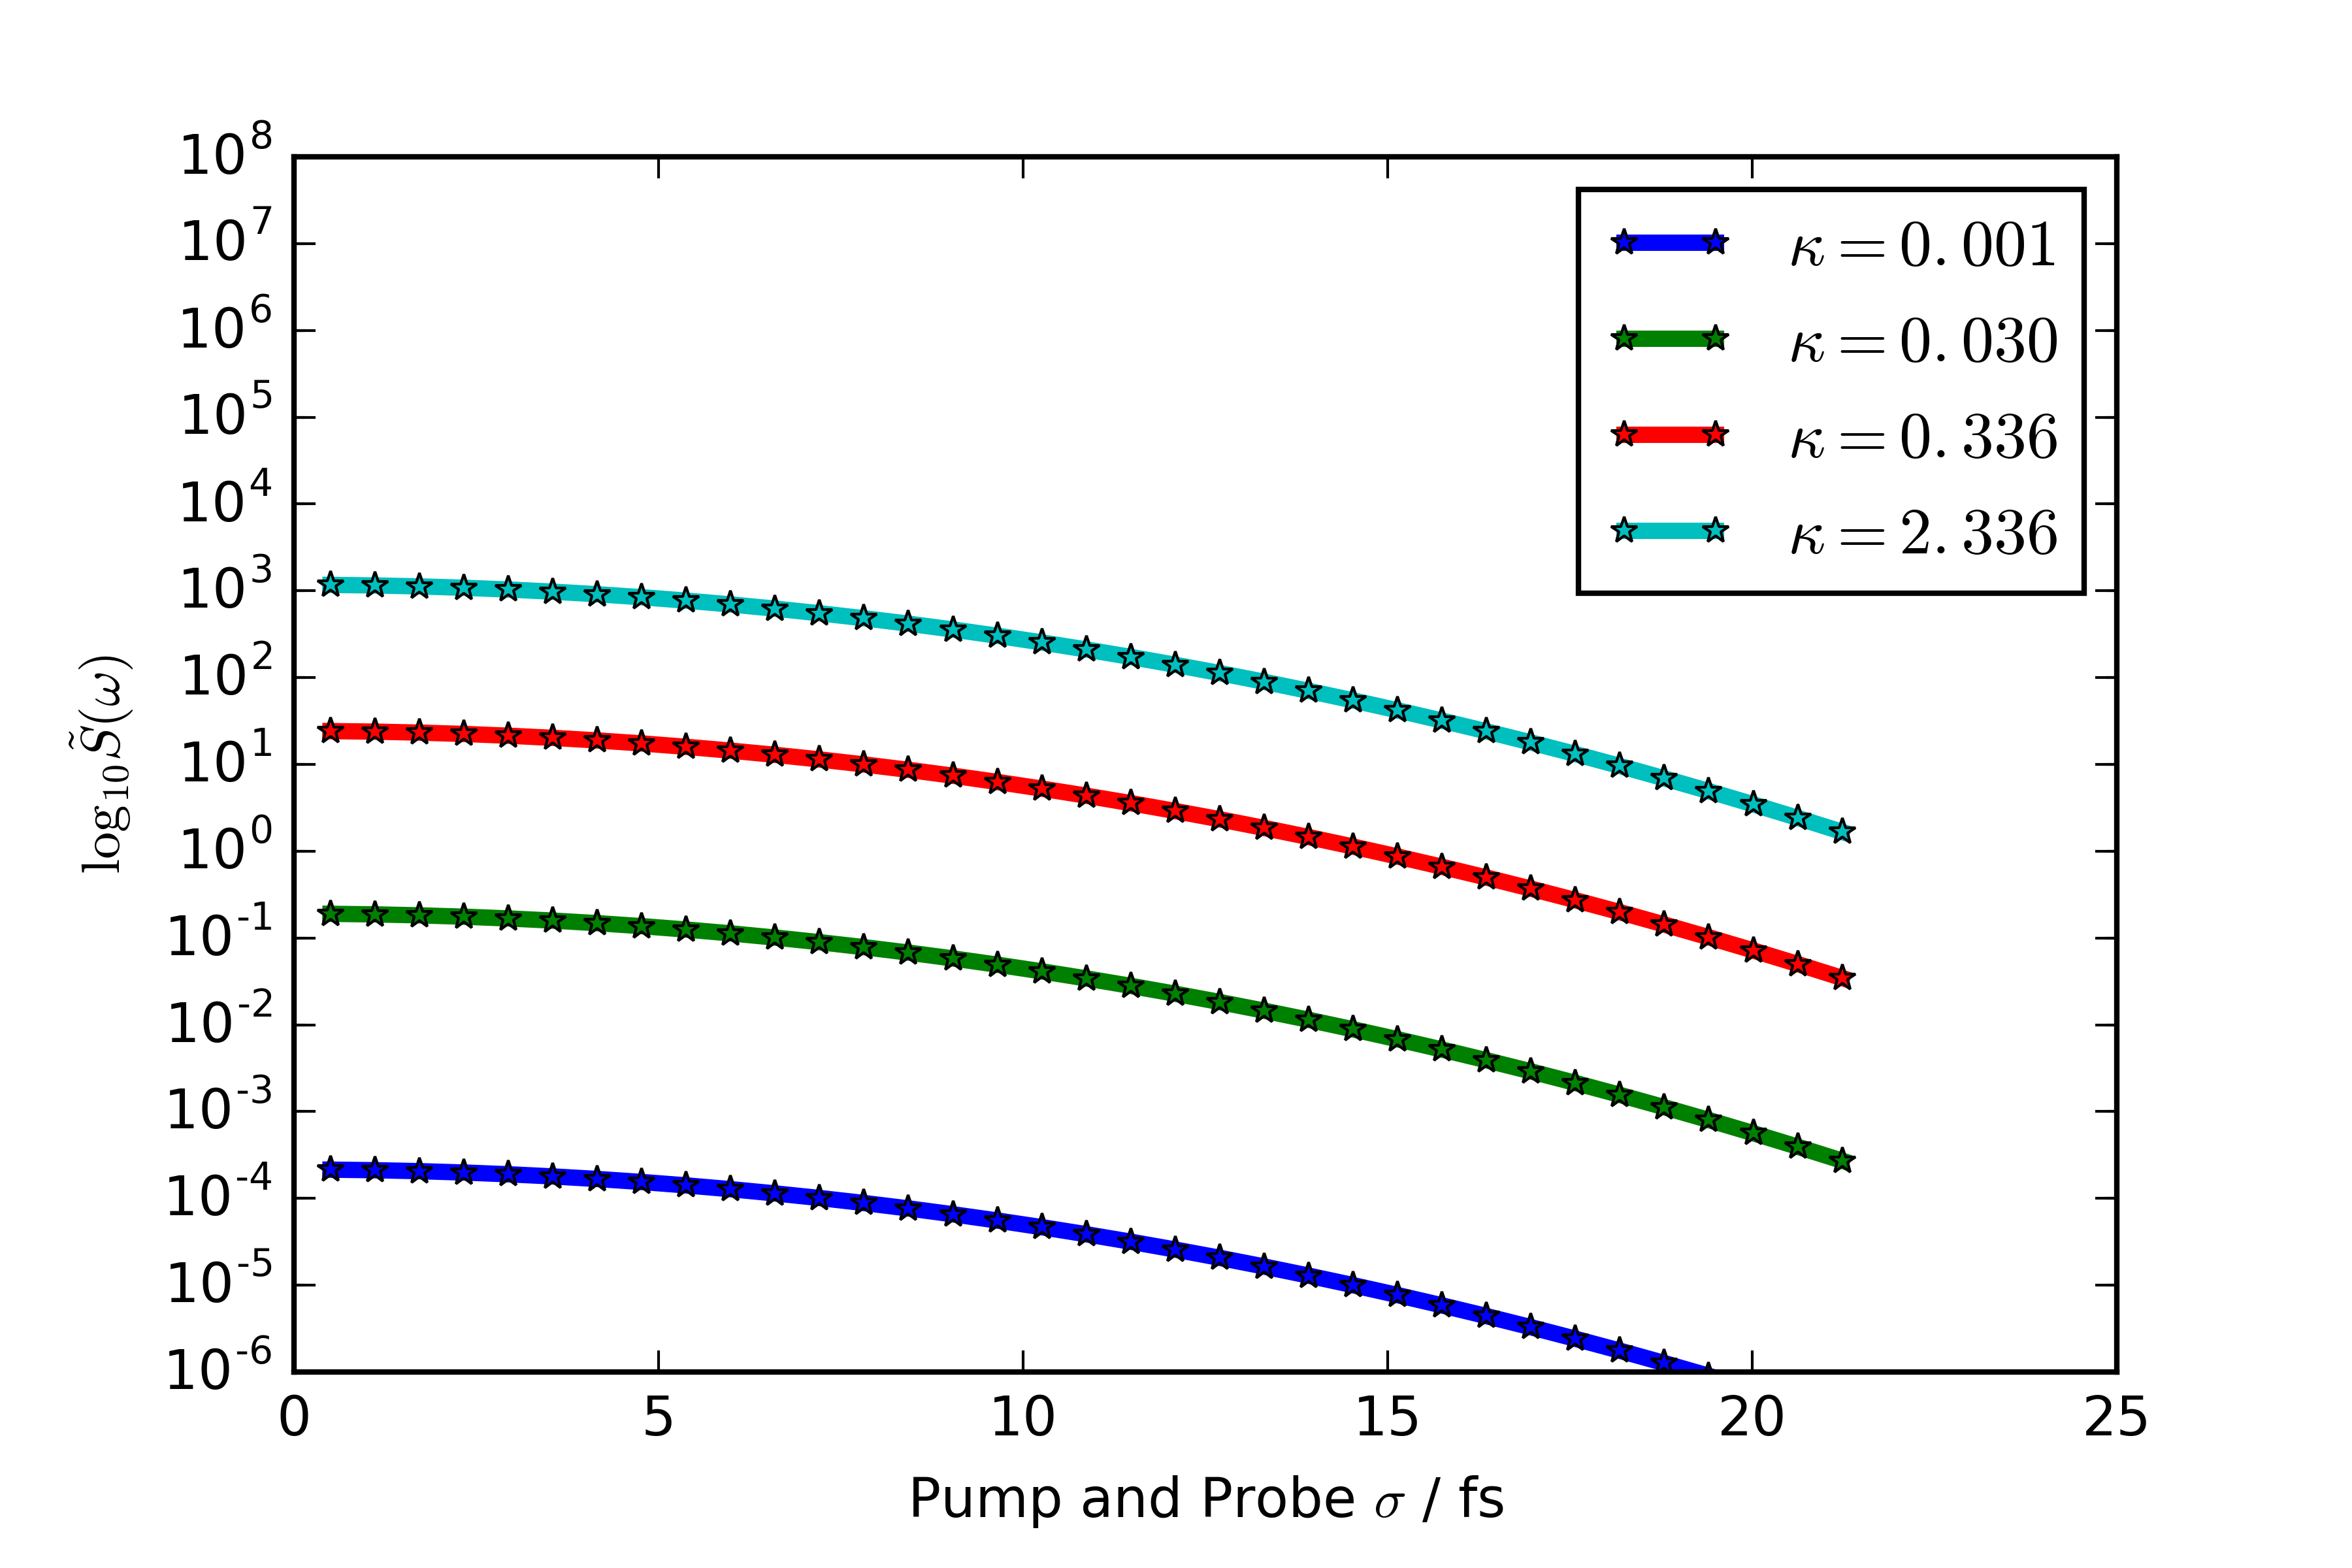
\includegraphics[width=1.0\columnwidth]{S0_samefrequency_kappa_comparison.png}
   \caption{Pump-probe oscillations at the vibrational frequency, $\tilde{S}_{PP} ( \omega)$, for a system with $S=0$ and $\omega_{\gamma} = \omega_{\epsilon} = \omega = $ 640 cm$^{-1}$, for various values of $\kappa$.  The signal is log scaled due to the signal's fourth-order dependence on $\mu(x)$; small differences in $\kappa$ make very large differences in signal.  In all of these systems, an experimenter using the proposed protocol would conclude that an electronic coherence exists in the system when there's not even a vibrational coherence in the ground state, absent a non-constant transition dipole. }
	\label{fig:tunedZero}
\end{figure}


We now consider $S=0.005$, which is close to photosynthetic Huang-Rhys factors ~\cite{typicalHRFforPhotosynthesis}, with results in Fig.\ \ref{fig:s_0p005}.  For this small $S$, the witness protocol essentially does not work for any $\lambda>10^{-3}$.

\begin{figure}
   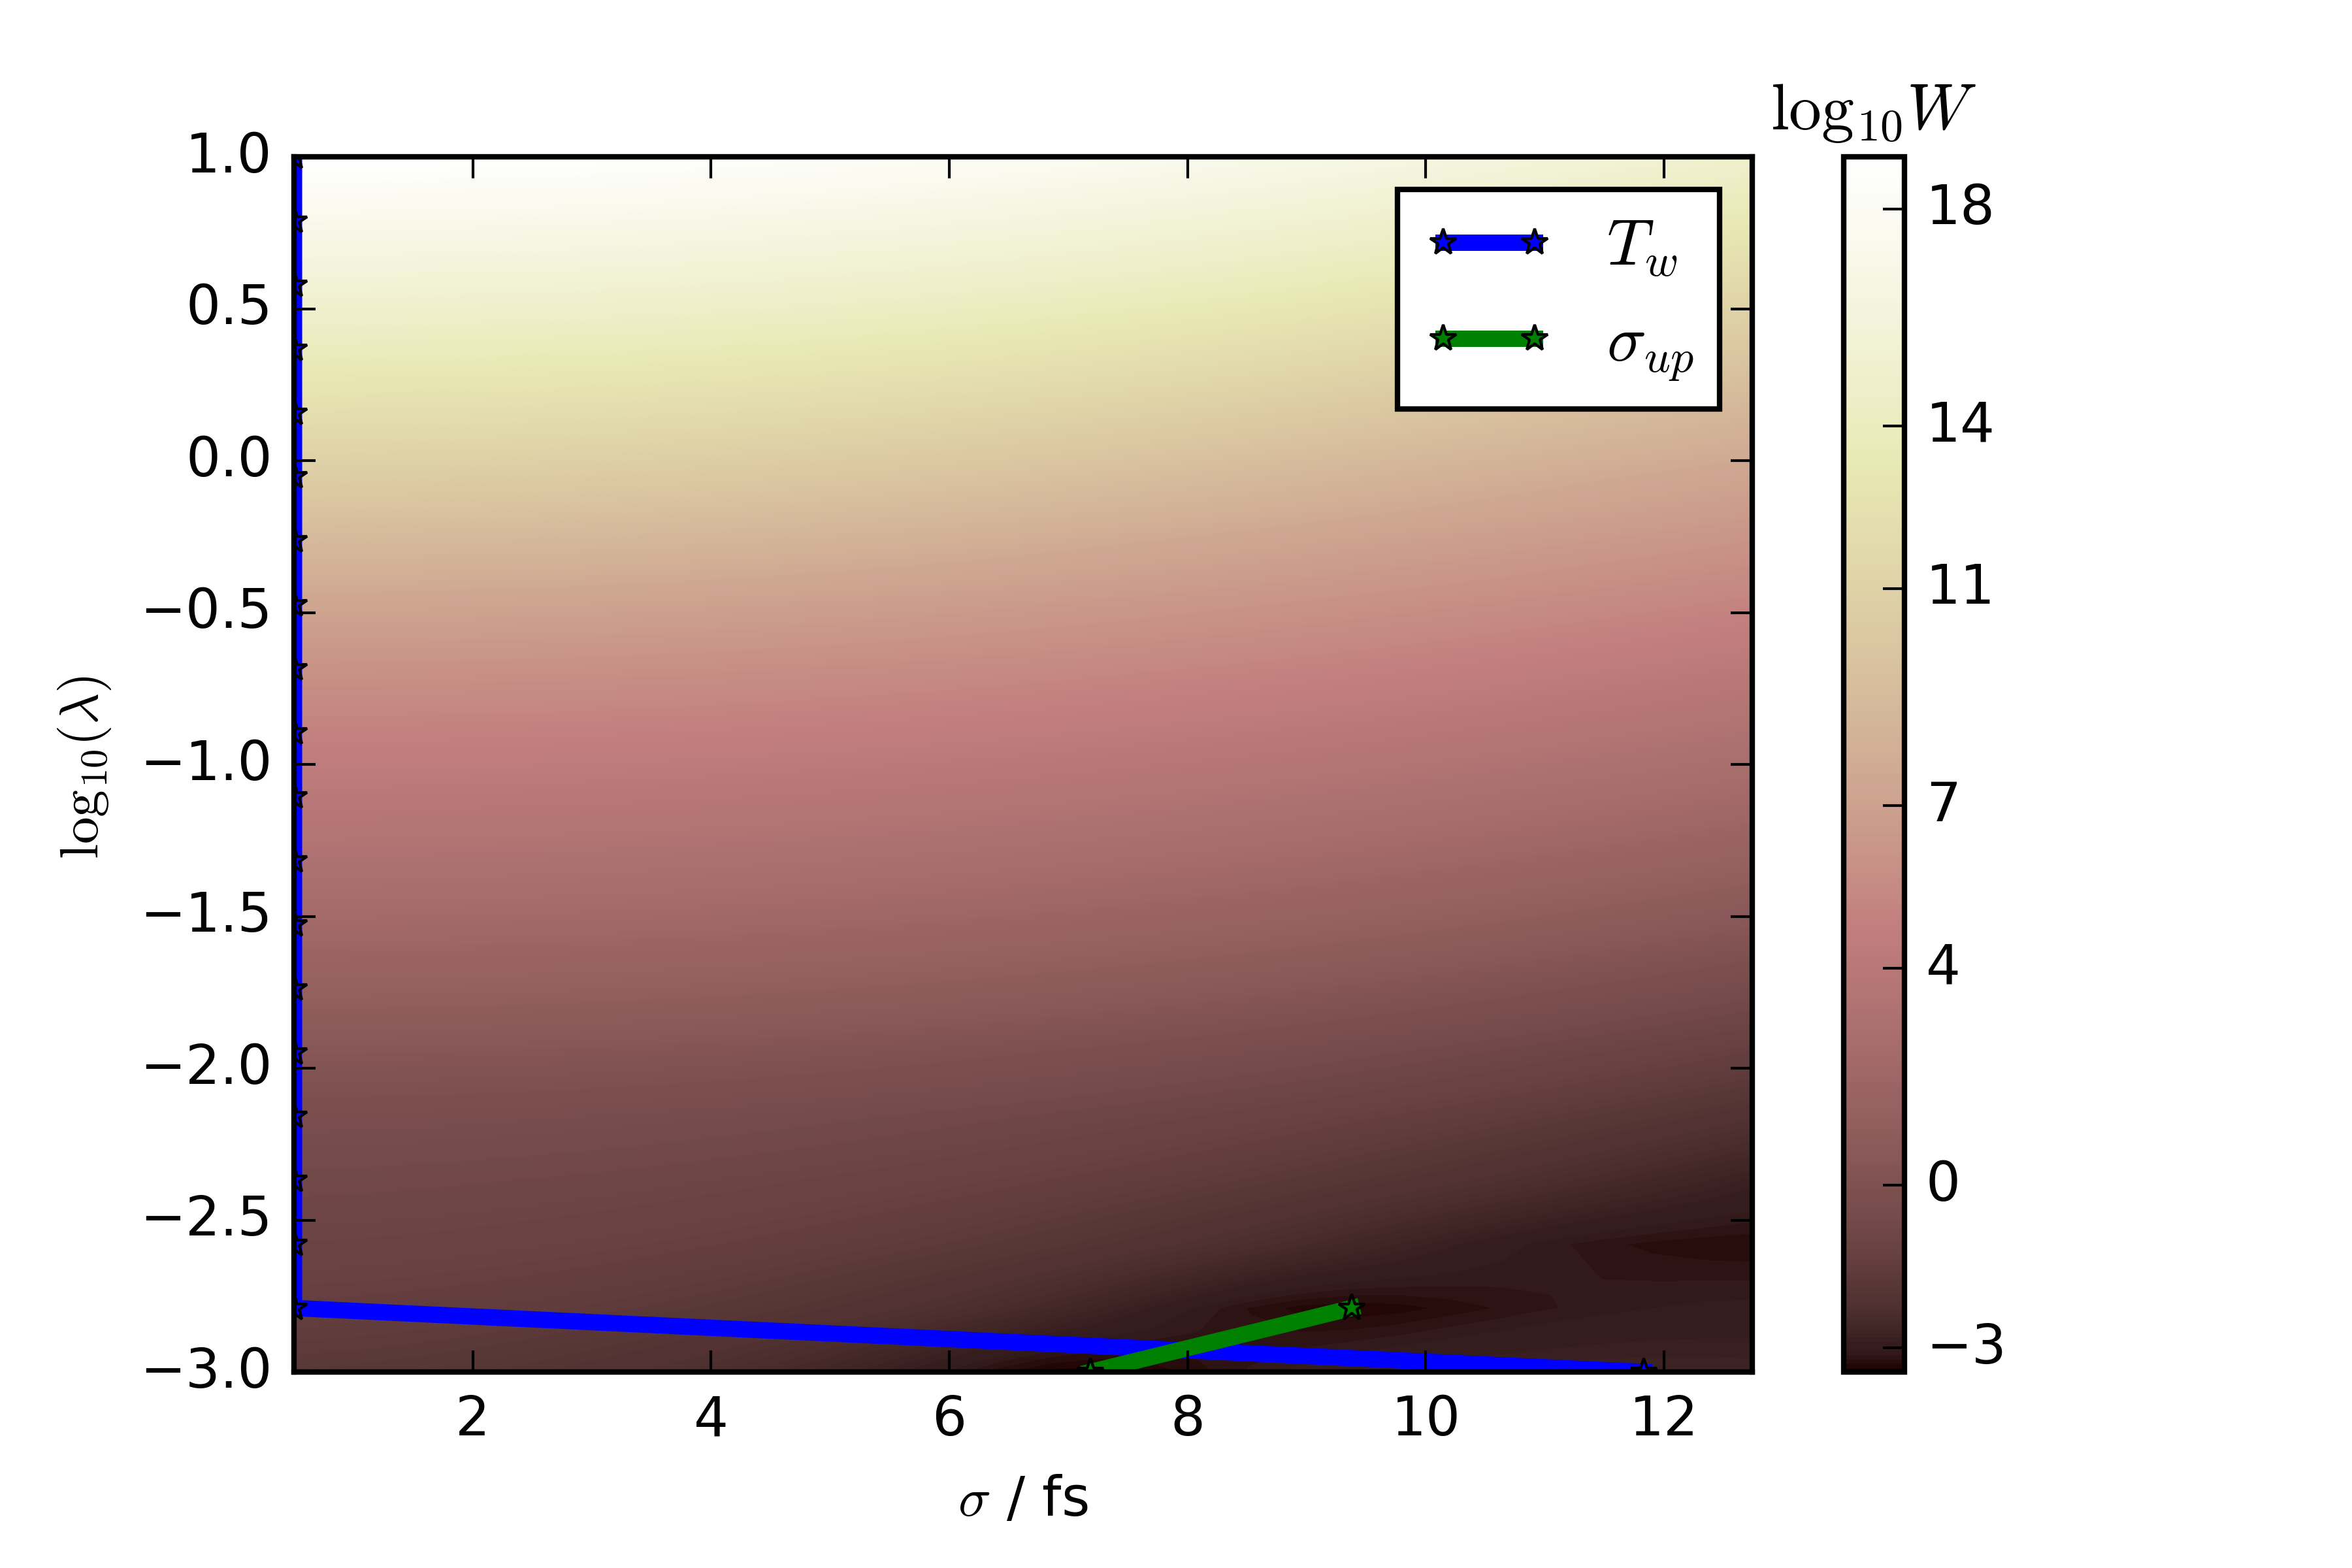
\includegraphics[width=1.0\columnwidth]{W_S_0p005_contour.png}
   % \caption{$\tilde{S}_{PP} ( \omega_e)$ as a function of $\lambda$ and the pulse width $\sigma$ in a system where $S=0.005$, $\omega_e = .9 \omega_g$. and $\omega_g = 640 \text{cm}^{-1}$. $T_w$ is the same as defined in reference \cite{allanWitness}: the peak of the signal before it goes down again.   Some traces in $\lambda$ have local minima as well when the signal goes up and we plot those as $\sigma_{up}$.  In the case where the signal just goes up as the pulse width goes down, then $T_w$ is set as $\sigma=0$.  }
   \caption{$\Gamma$ as a function of $\lambda$ and the pulse width $\sigma$ in a system where $S=0.005$, $\omega_e = .9 \omega_g$. and $\omega_g = 640 \text{cm}^{-1}$. $T_w$ is the same as defined in reference \cite{allanWitness}: the peak of the signal before it goes down again.   Some traces in $\lambda$ have local minima as well when the signal goes up and we plot those as $\sigma_{up}$.  In the case where the signal just goes up as the pulse width goes down, then $T_w$ is set as $\sigma=0$.  }
	\label{fig:s_0p005}
\end{figure}

We now consider $S=0.2$, with results in Fig.\ \ref{fig:s_0p2}. For this larger value of $S$, for $\lambda<0.1$, the witness signature is apparent in the data, with a declining pump-probe signal as $\sigma$ is reduced, until the pulse duration $\sigma_{up}$ is reached. For $\sigma<\sigma_{up}$, the signal again increases, due to the non-Condonicity. This upturn occurs at short pulse durations, after the usual peak structure of a negative witness is well established, coming from large $\sigma$ to $T_w$ down to $\sigma_{up}$.

We propose a modified witness protocol that declares a negative witness (i.e., vibrational-only coherence) in experiments that observe a peak at $T_w$ and a short-duration upturn at $\sigma_{up}$. We consider such a structure to be observed if the signal $\tilde{S}_{PP}(\omega)$ at $T_w$ is more than twice the value of the signal at $\sigma_{up}$, and we call this ratio $w$. In such a case, the experiment has determined both the vibrational character of the relevant coherence as well as the presence of a non-Condon contribution to the transition dipole. Further methods for detecting and measuring non-Condon transition dipoles can be found in Ref.\  ~\cite{myDetectingNonCondonPaper}.

With this modified protocol in mind, we construct figure \ref{fig:working_regions_W} where we show the ratio $w$ for 5 values of $S$.  With our criteria that $w \leq 0.5$ there are quite a few regions where the proposed protocol will still work, but even more where it will give false positives.

\begin{figure}
   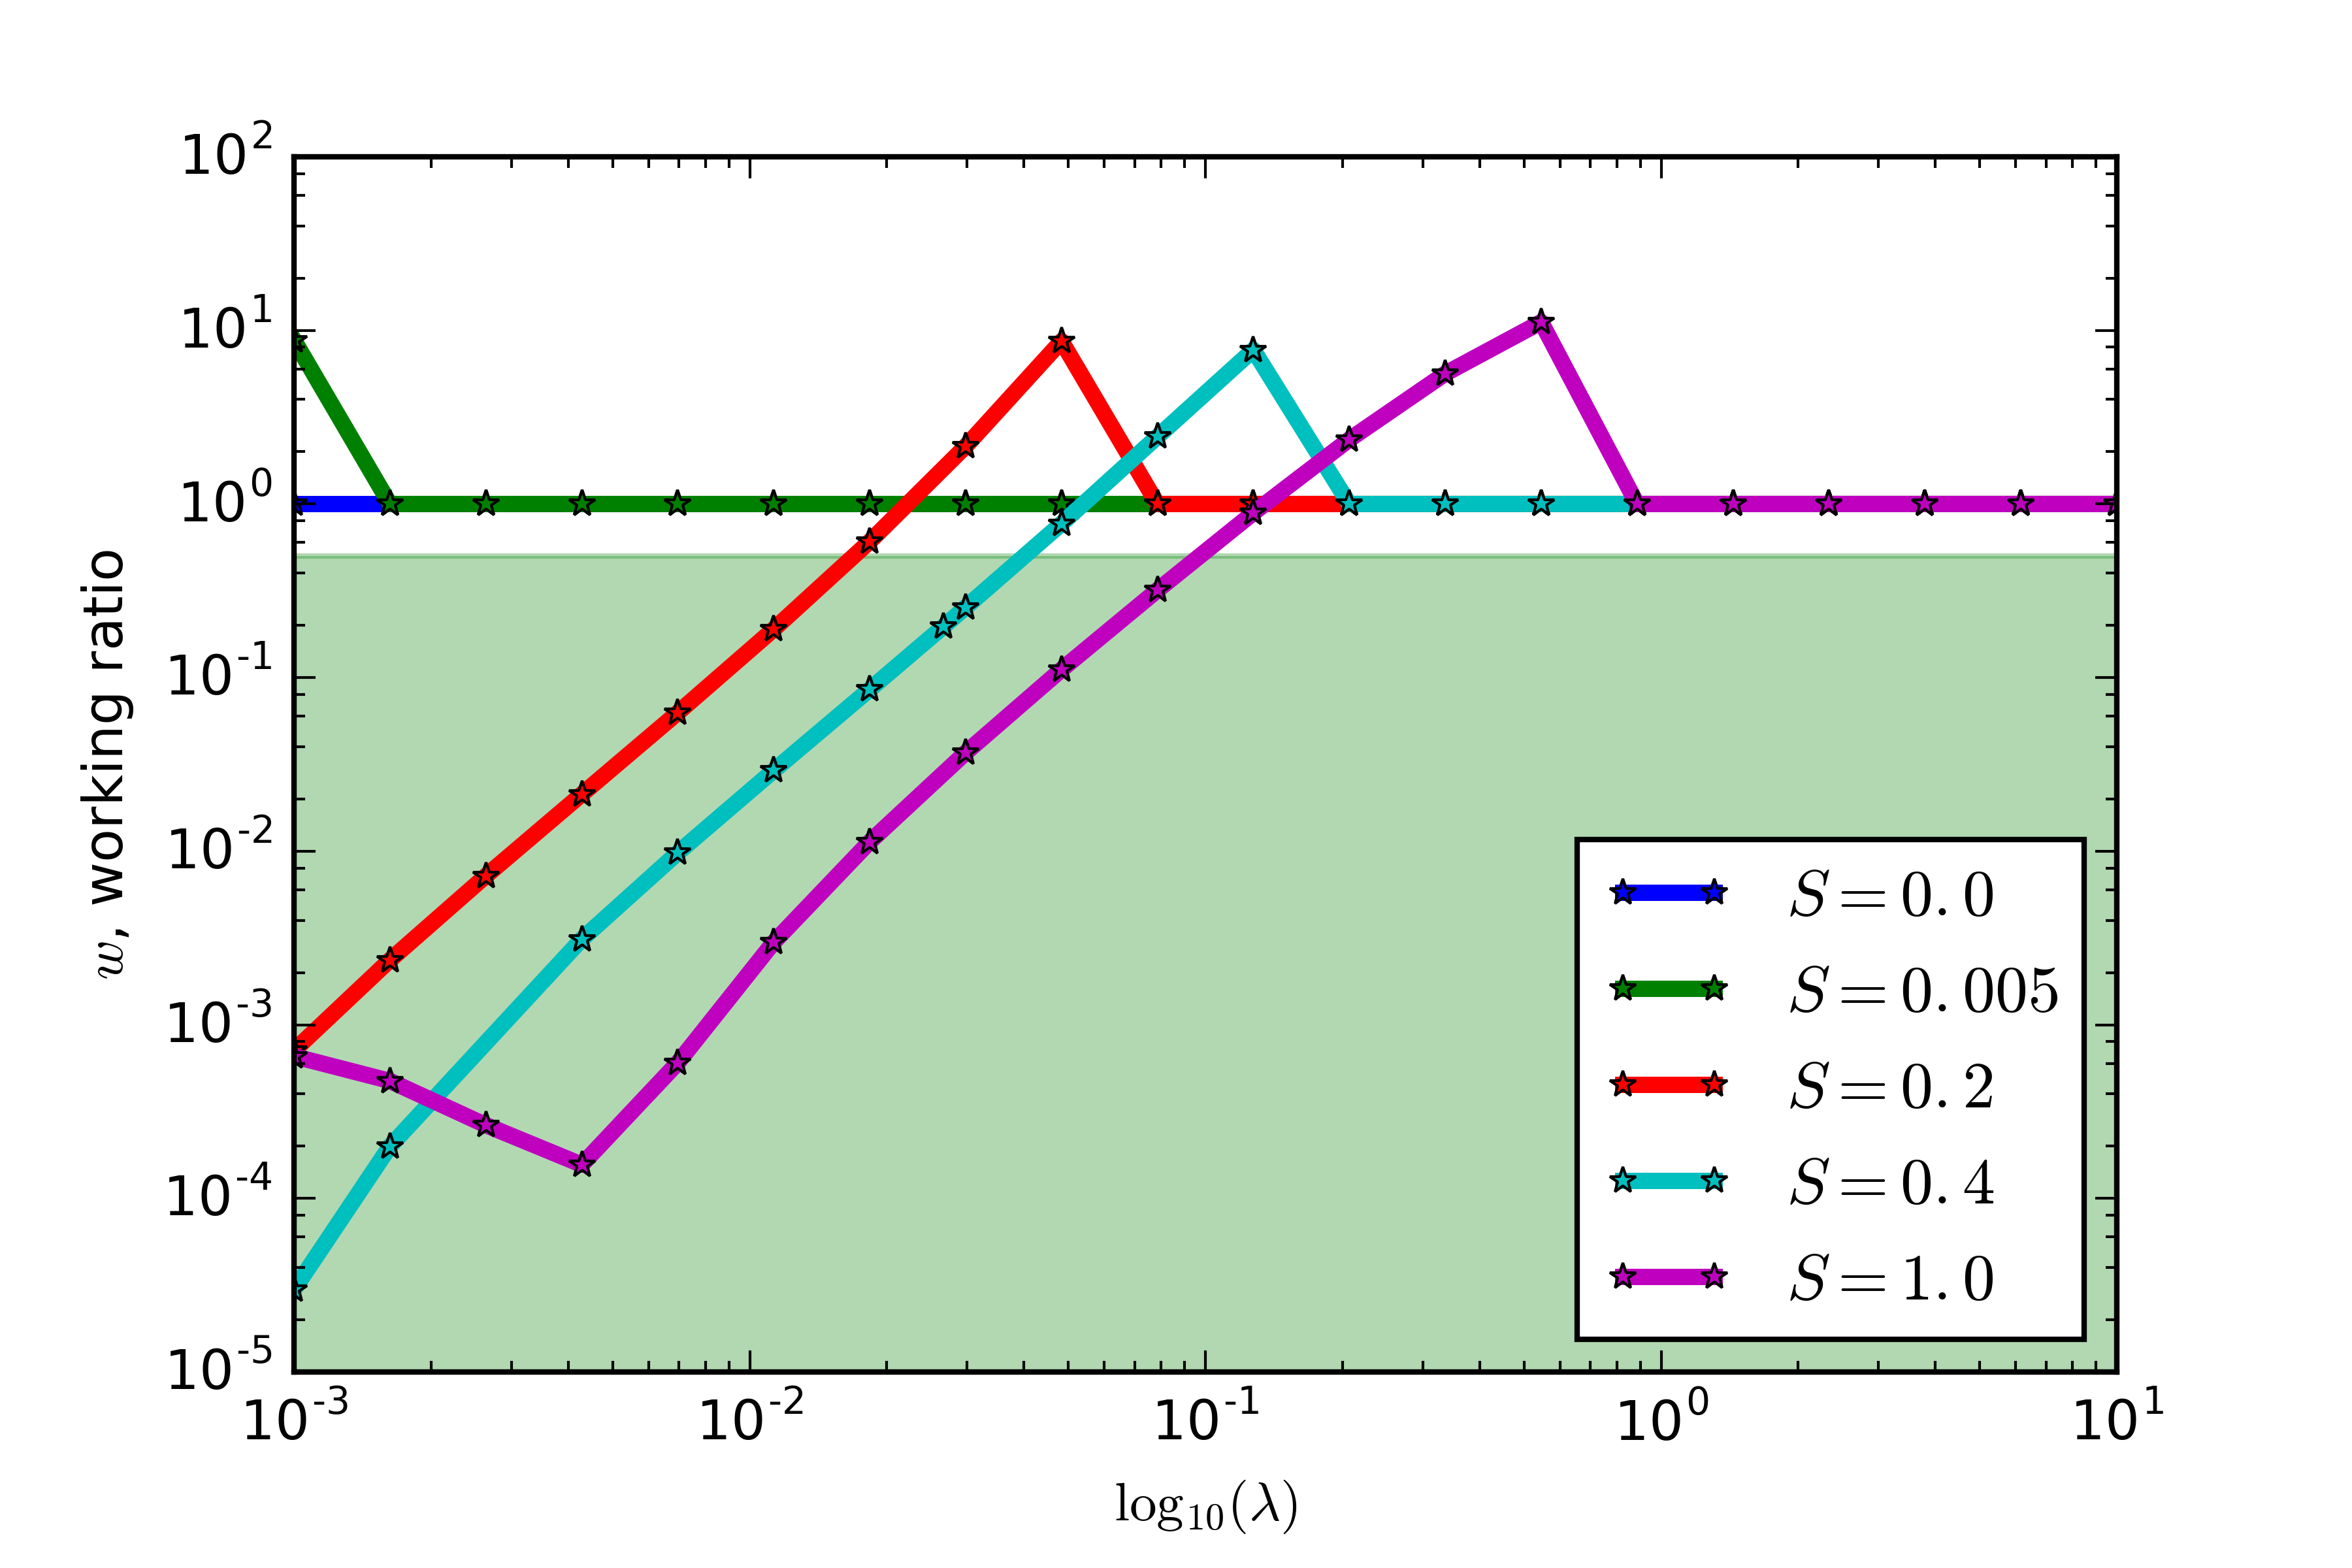
\includegraphics[width=1.0\columnwidth]{working_regions_W.png}
   \caption{The ratio $w$ of the oscillation amplitude at the minimum pulse width to the oscillation amplitude at the local maxima (or witness time $T_w$) for various values of $S$.  The region shaded in green is where our modified protocol does not produce a false-positive. }
	\label{fig:working_regions_W}
\end{figure}

Reference \cite{allanWitness} proposed using the entire frequency-integrated pump-probe signal $\Gamma=\int |S_{PP}(T)-\bar{S}_{PP}|^2 dT$, where $\bar{S}_{PP}$ is the average value of the pump-probe signal and the integral is taken only for $T>3\sigma_{max}$, to avoid pulse-overlap effects, where $\sigma_{max}$ is the largest pulse duration studied in the experiment. In this work we have considered the frequency-resolved pump-probe signal $\tilde{S}_{PP}(\omega)$, but the analysis for $\Gamma$ is similar and gives the same regions of $(S,\lambda)$ where the modified witness protocol functions.

\begin{figure}
   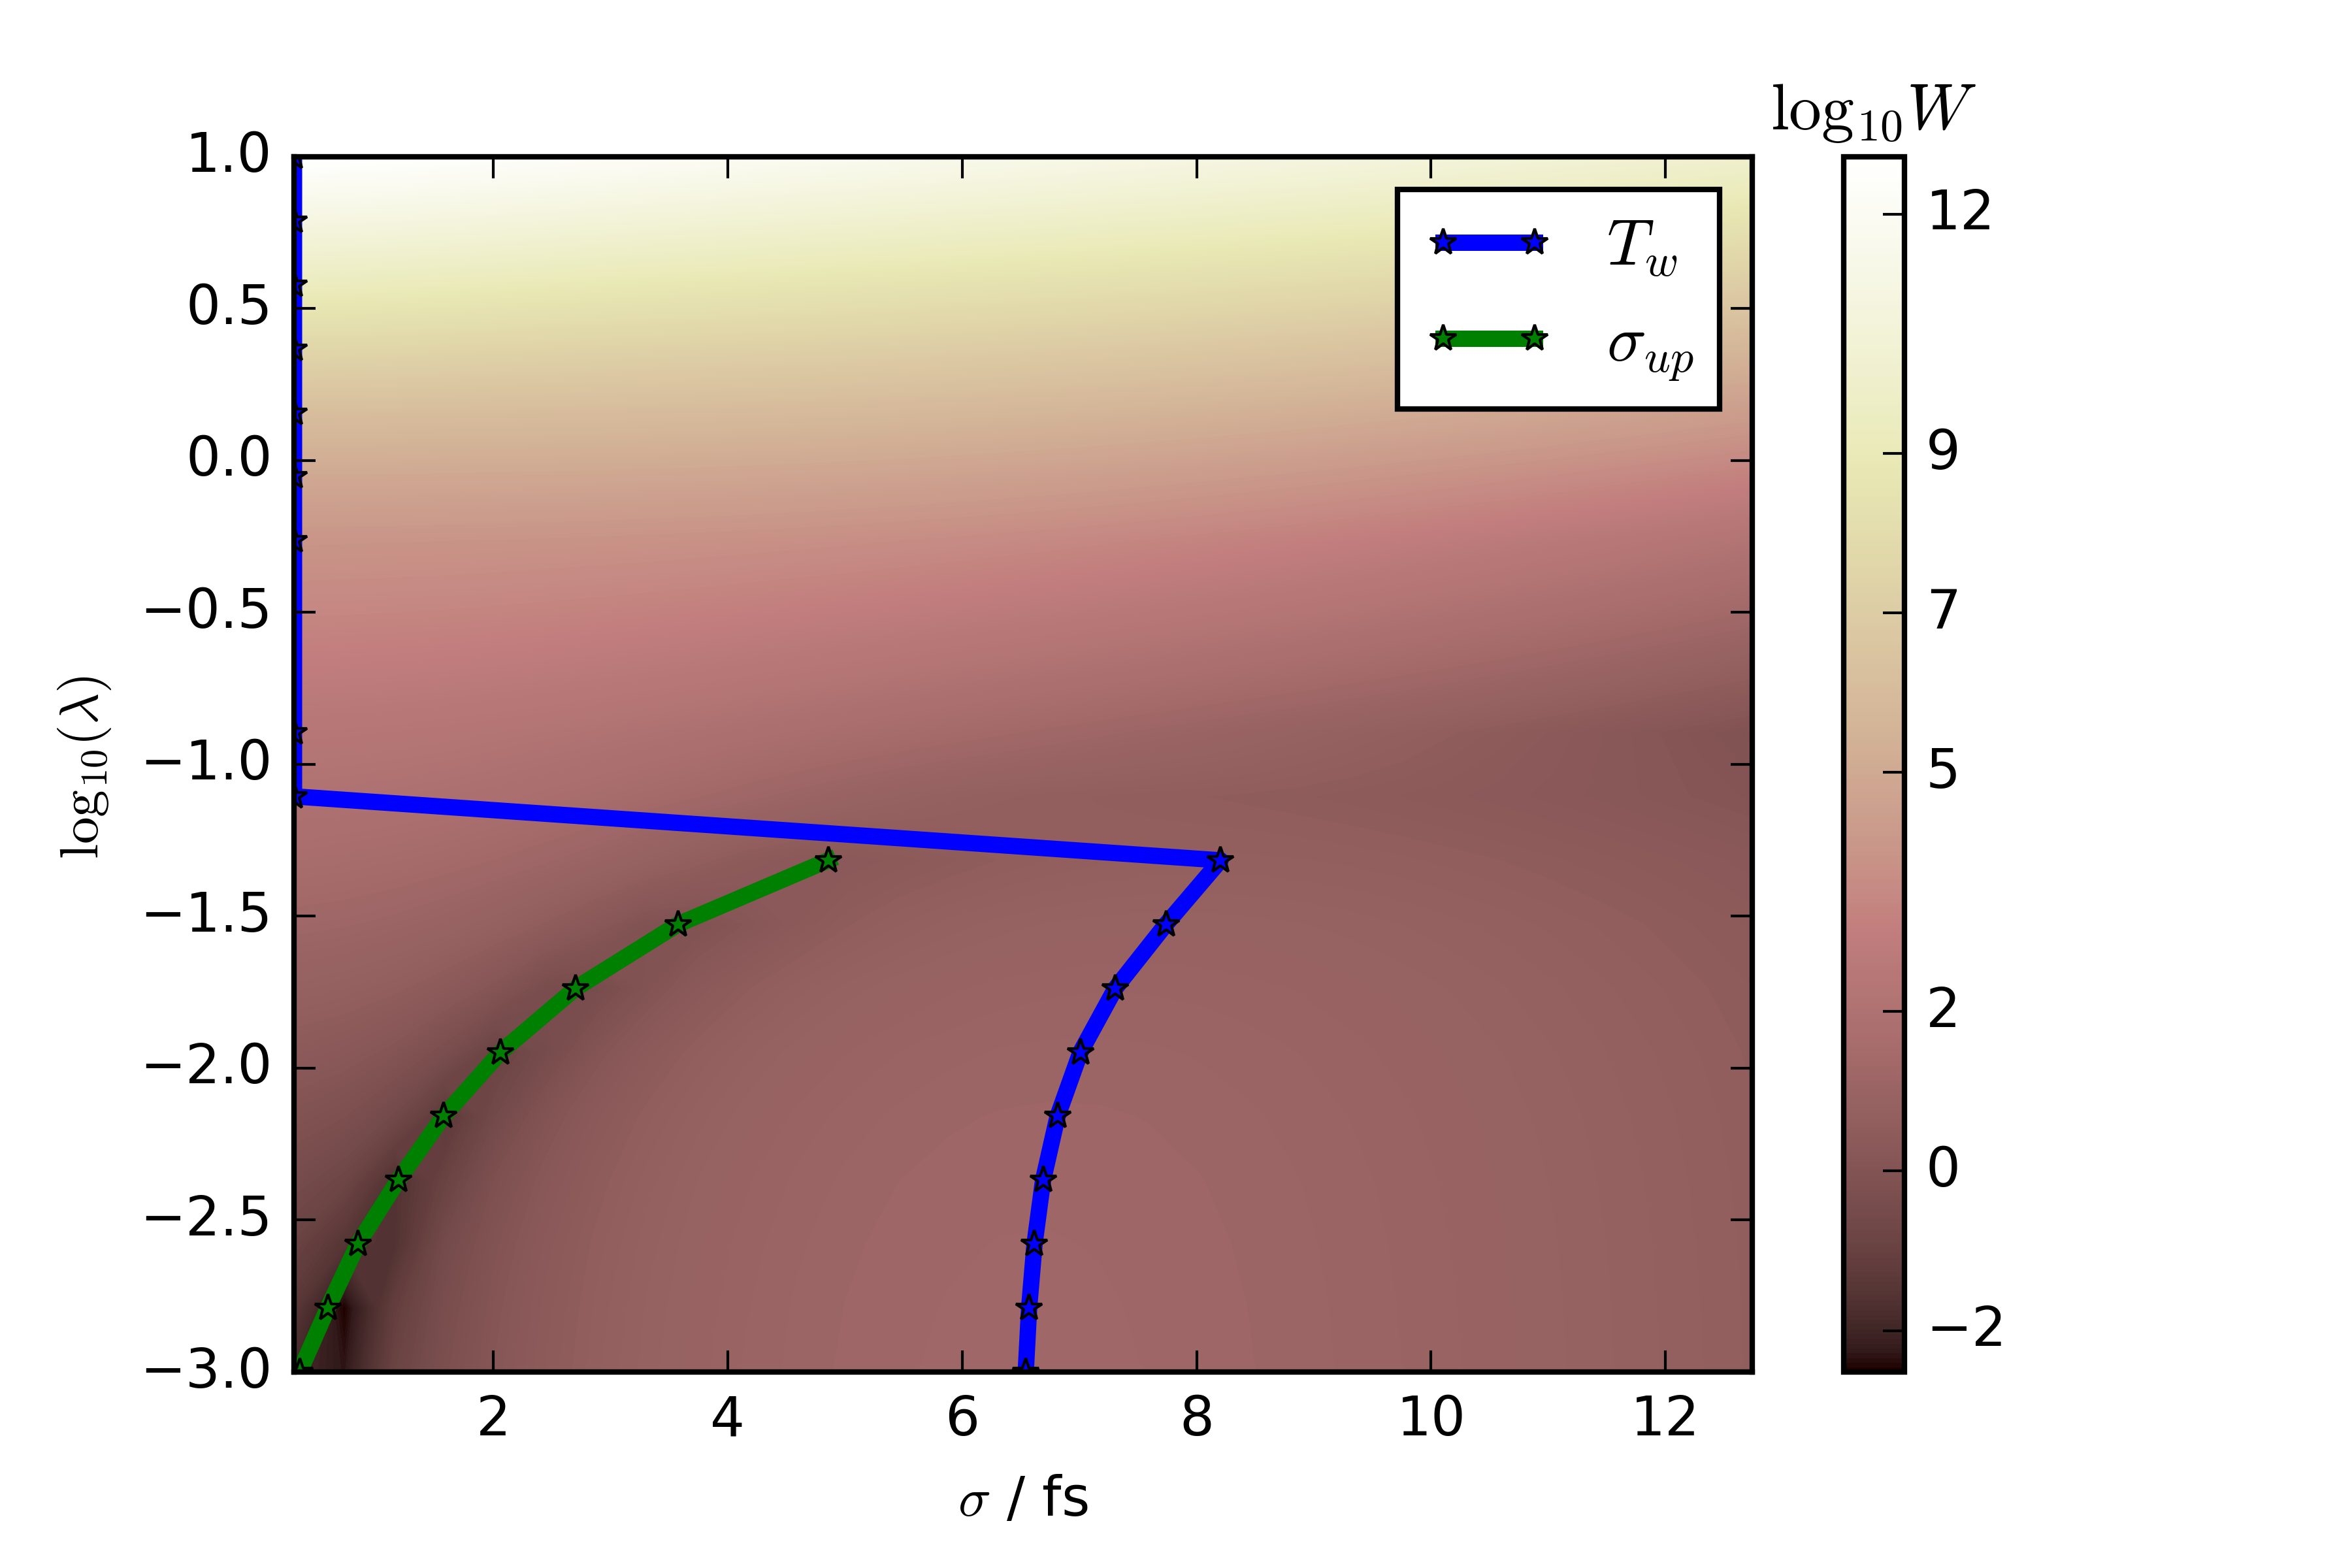
\includegraphics[width=1.0\columnwidth]{W_S_0p2_contour.png}
   \caption{$\Gamma$ as a function of $\lambda$ and the pulse width $\sigma$ in a system where S=0.2, $\omega_e = .9 \omega_g$. and $\omega_g = 640 \text{cm}^{-1}$.  }
   % \caption{$\tilde{S}_{PP} ( \omega_e)$ as a function of $\lambda$ and the pulse width $\sigma$ in a system where S=0.2, $\omega_e = .9 \omega_g$. and $\omega_g = 640 \text{cm}^{-1}$. \textbf{Add a part (b) to this figure with three line cuts at $\lambda=0.001,0.01,0.1$?} }
	\label{fig:s_0p2}
\end{figure}

\begin{figure}
   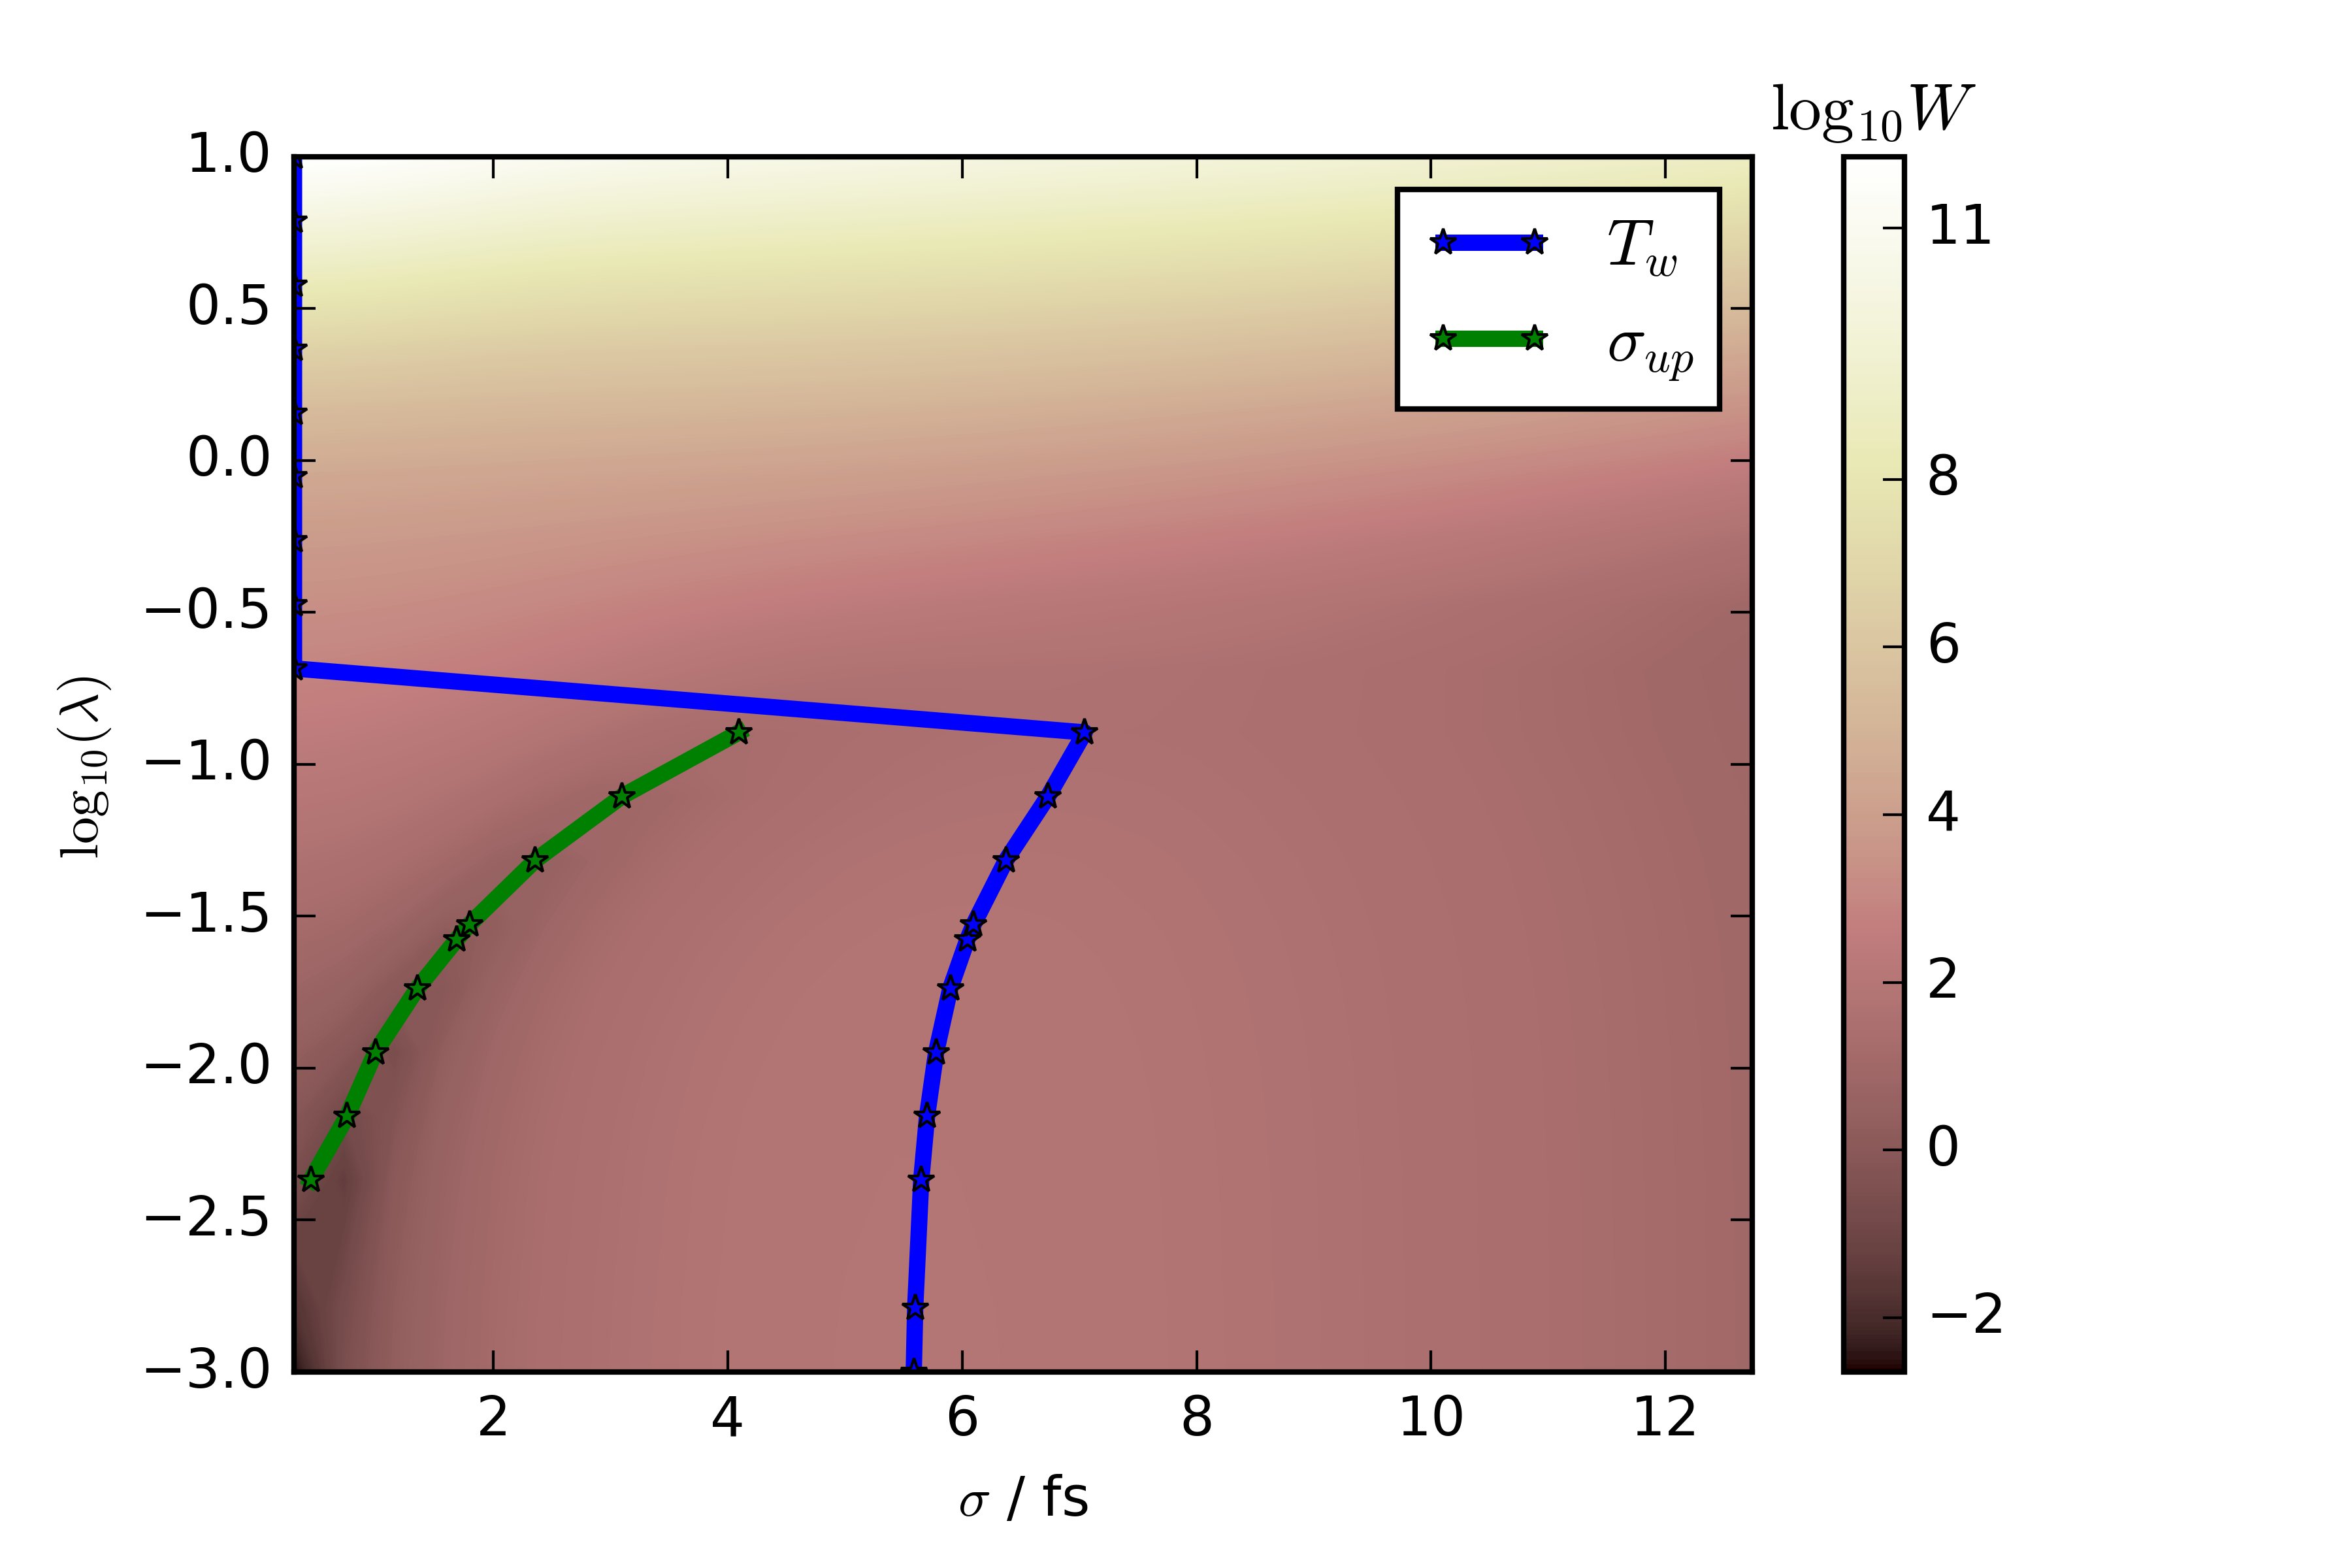
\includegraphics[width=1.0\columnwidth]{W_S_0p4_contour.png}
   \caption{$\Gamma$ as a function of $\lambda$ and the pulse width $\sigma$ in a system where $S=0.4$. $\omega_e = .9 \omega_g$. and $\omega_g = 640 \text{cm}^{-1}$.}
   % \caption{$\tilde{S}_{PP} ( \omega_e)$ as a function of $\lambda$ and the pulse width $\sigma$ in a system where $S=0.4$. $\omega_e = .9 \omega_g$. and $\omega_g = 640 \text{cm}^{-1}$.}
	\label{fig:s_0p4}
\end{figure}

\begin{figure}
   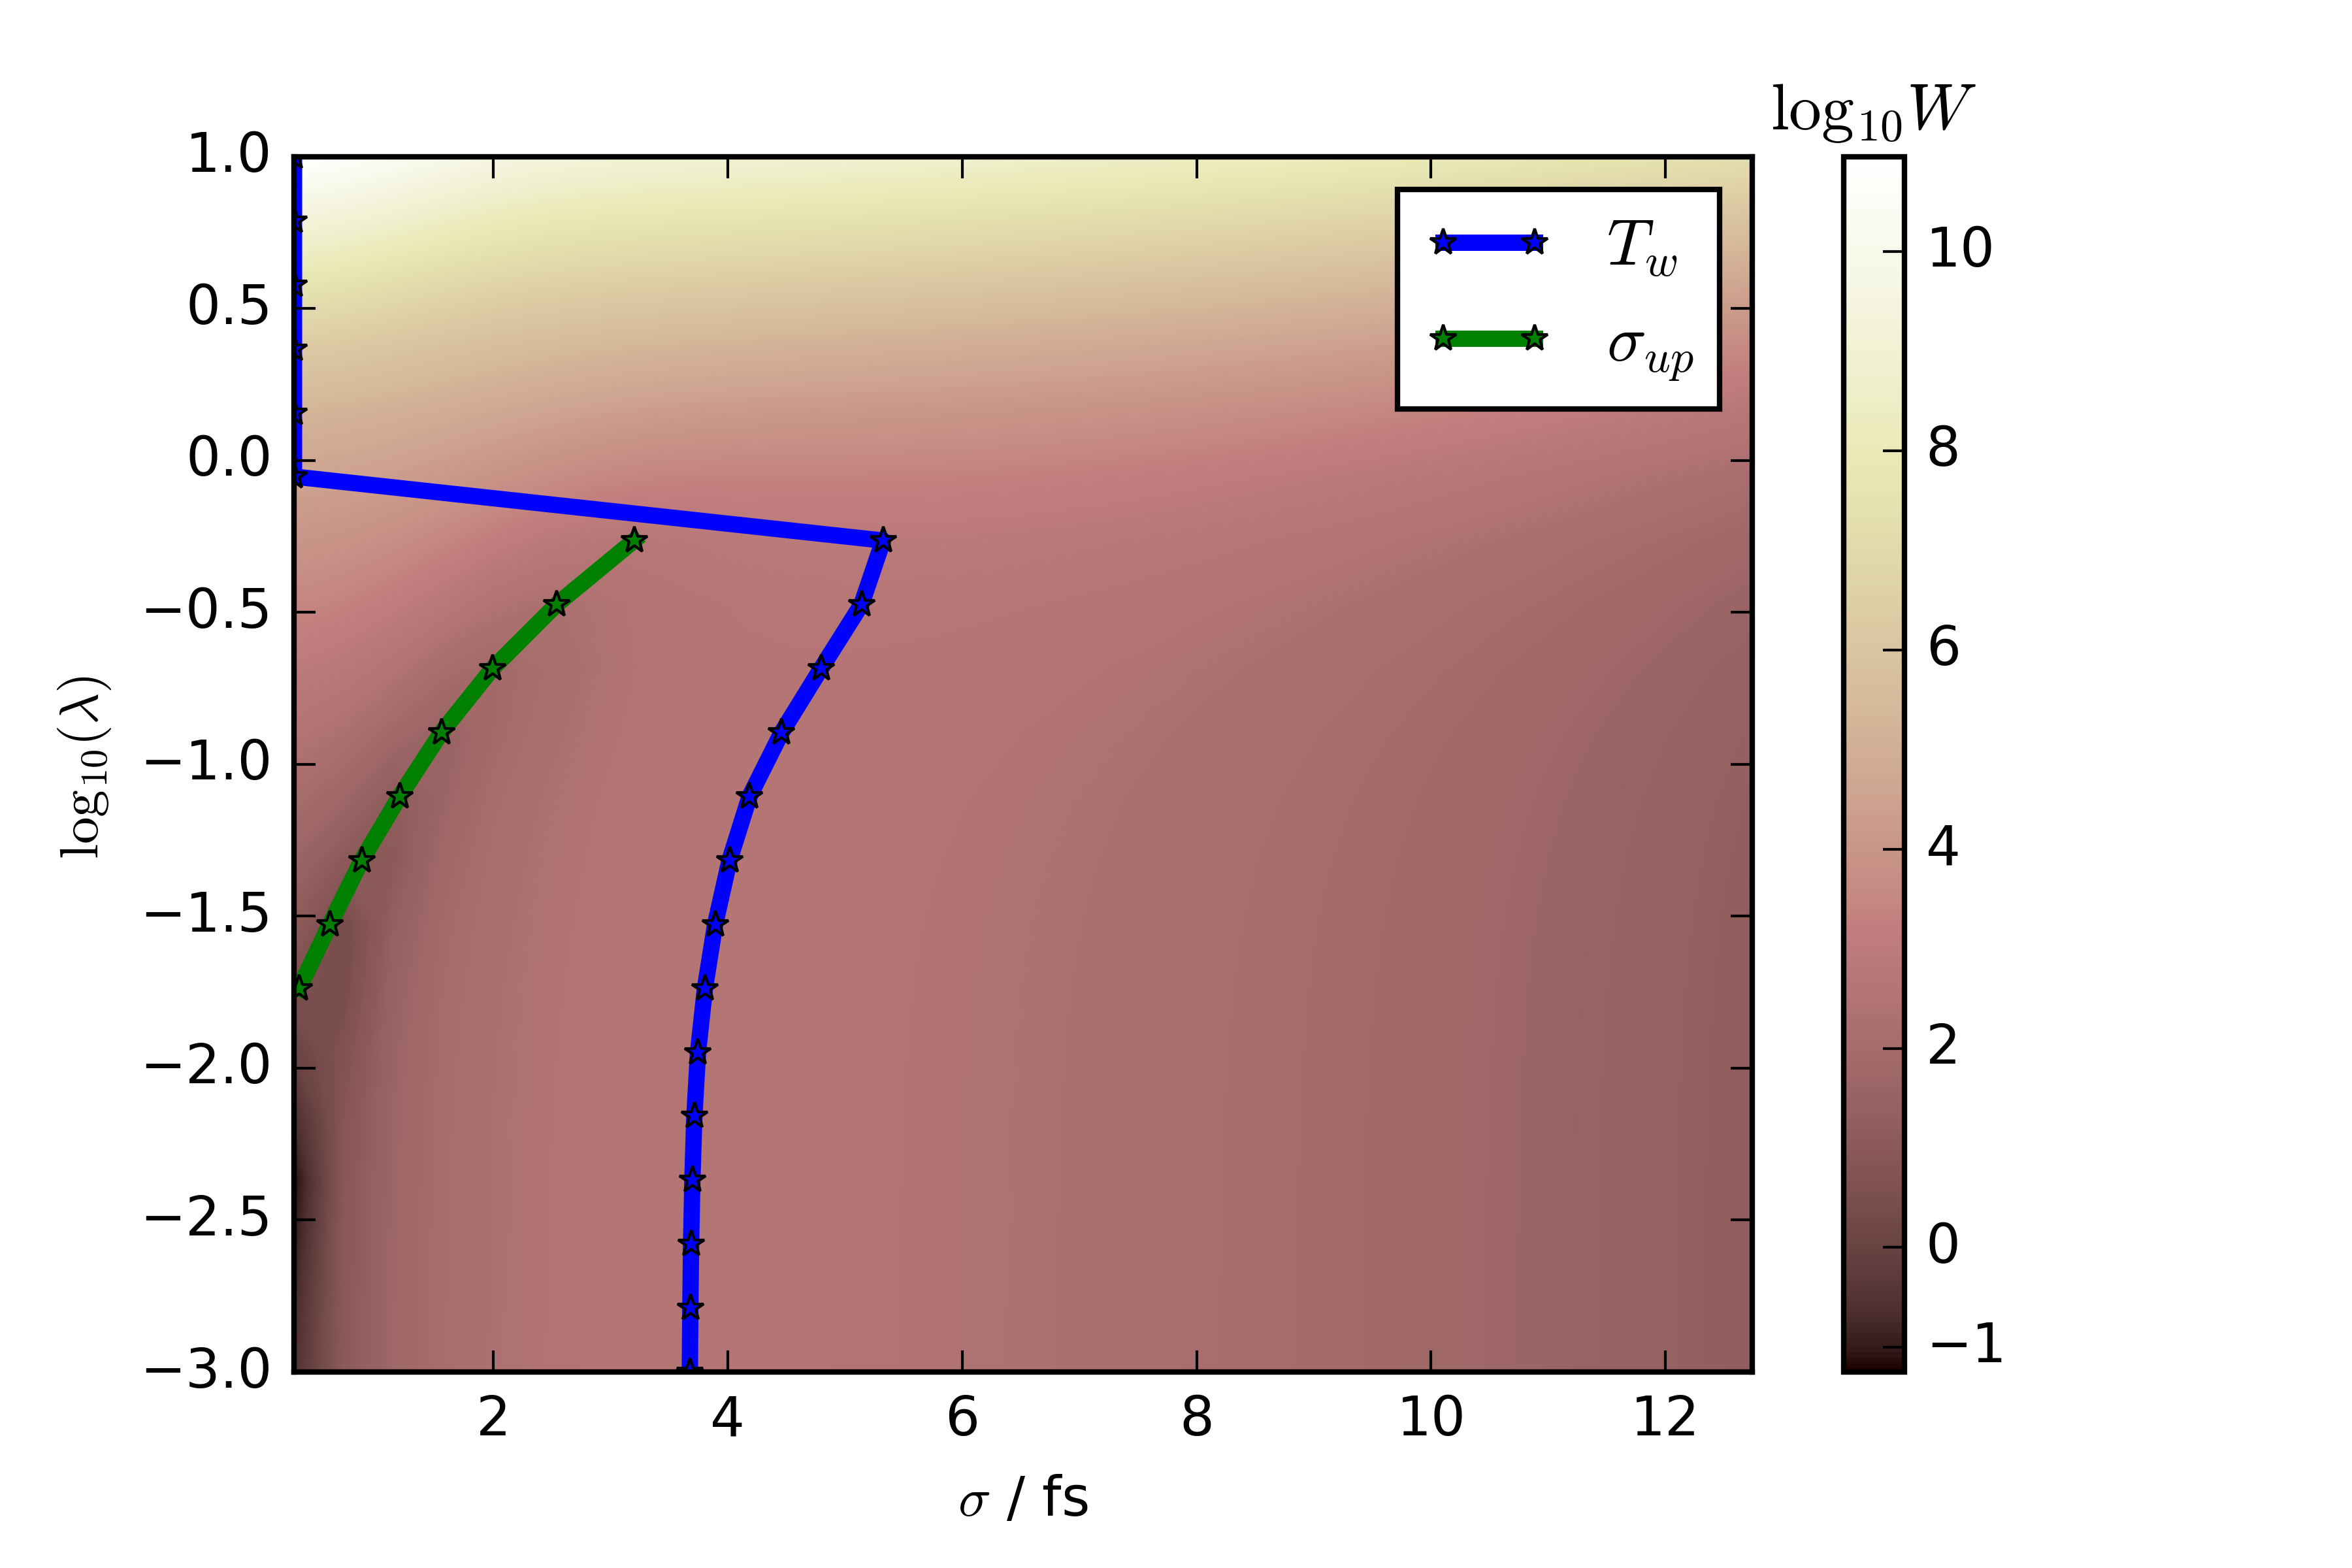
\includegraphics[width=1.0\columnwidth]{W_S_1p0_contour.png}
   \caption{$dT$ as a function of $\lambda$ and the pulse width $\sigma$ in a system where $S=1.0$, $\omega_e = .9 \omega_g$. and $\omega_g = 640 \text{cm}^{-1}$. }
   % \caption{$\tilde{S}_{PP} ( \omega_e)$ as a function of $\lambda$ and the pulse width $\sigma$ in a system where $S=1.0$, $\omega_e = .9 \omega_g$. and $\omega_g = 640 \text{cm}^{-1}$. }
	\label{fig:s_1p0}
\end{figure}

To investigate the dips in signal seen in figures \ref{fig:s_0p005} and \label{fig:s_0p2}, we introduce figure \ref{fig:addedSignals}, where we look at $S=.2$ and $\kappa=.037$.   When the nonzero $\kappa$ is turned off and set to zero, we get a decreasing oscillatory signal approaching zero as the laser pulse width approaches zero just as predicted by ~\cite{allanWitness}.  If, however, we turn on the nonzero $\kappa$, we see the while there is a dip at a certain point in the signal, it increases as the pulse width approaches zero.  Indeed, even if we set $S=0.0$ but keep the same value of $\kappa$, and thus have a system that should have almost no oscillations, there is still an increasing oscillation signal.  The shape of these three curves suggests that there is an interference interplay between the tendency of a vibrational coherence to go down as the pulse width approaches zero and the tendency of an oscillation induced by a linear transition dipole variation to increase as the pulse width gets toward zero.

\begin{figure}
   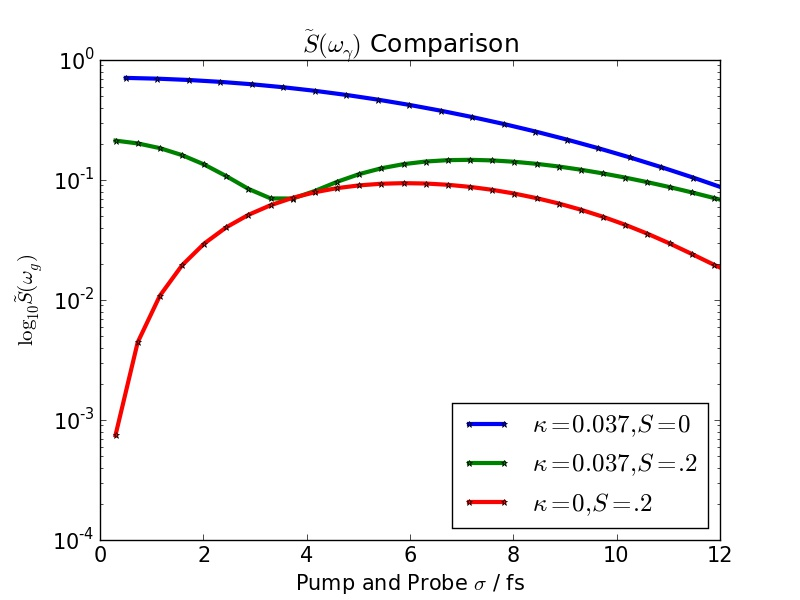
\includegraphics[width=1.0\columnwidth]{comparison_omega_g.jpg}
   \caption{$\tilde{S}_{PP} ( \omega_{\gamma})$ Here we have plotted the ground state oscillations for 3 systems: $\kappa=.037, S=0$; $\kappa=.037, S=0.2$; and $\kappa=0.0, S=0.2$.  This shows roughly that the effects of a non-Condon monomer without vibrational displacement add together with the effects of a Condon monomer to get the result for a non-Condon monomer with a vibrational displacement}
	\label{fig:addedSignals}
\end{figure}




\section{Conclusion}

The proposed witness for electronic coherences \cite{witness,allanWitness} relied on the Condon approximation. We have found that in vibrational systems with very small Huang-Rhys factors $S$, small non-Condon effects can give false-positive effects, where a system with no electronic coherence is incorrectly determined to have an electronic coherence. For larger $S$, the witness protocol can be successfully used for larger values of $\lambda$. It is possible that modified experimental procedures could increase the domain of ($S$, $\kappa$) in which the witness protocol will function. In order to apply the witness protocol, one must be able to estimate or measure the non-Condon effects to be sufficiently small. Methods to measure non-Condonicity are proposed in Ref. \cite{myDetectingNonCondonPaper}.




\section{Acknowledgments}
We acknowledge support from the Center for Excitonics, an Energy Frontier Research Center funded by the U.S. Department of Energy under award DE-SC0001088 (Solar energy conversion process) and the Natural Sciences and Engineering Research Council of Canada.  The authors also wish to thank Doran Bennet for his useful commentary on this manuscript.
